\documentclass[a4paper,man,natbib]{apa6}
\usepackage{microtype}
\usepackage{mathtools} % needed
\usepackage{hyperref}
\usepackage{tabularx}
\usepackage{lingex}
\usepackage[modulo,displaymath,pagewise]{lineno}

\newcolumntype{Y}{>{\raggedright\arraybackslash}X}
\usepackage[normalem]{ulem}
\hypersetup{hidelinks=True}
\newcommand*{\smex}[1]{\textit{#1}} % 'small example'
\newcommand*{\spex}[1]{``{#1}''} % 'spoken example'
\newcommand*{\term}[1]{\emph{#1}} % introducing a new term
\newcommand*{\citegen}[1]{\citeauthor{#1}'s~(\citeyear{#1})}
\newcommand*{\SE}{\mathit{SE}} % fix funny "SE" spacing
\newcommand{\resultsLog}[3]{$\beta = #1$, $\textnormal{SE} = #2$, $p #3$}
\newcommand{\resultsLM}[3]{$\beta = #1$, $\textnormal{SE} = #2$, $t #3$}

\usepackage[obeyFinal,textsize=tiny,backgroundcolor=yellow!60,linecolor=black!60]{todonotes} % to get rid of all notes, pass
% `final' to the document class
\setlength{\marginparwidth}{2cm}
\let\oldtodo\todo
\renewcommand*{\todo}[1]{\oldtodo[fancyline]{#1}}

\title{Interpreting nonverbal cues to deception in real time}
\shorttitle{Nonverbal Cues to Deception}

\author{reorder(MC,JK,JL)}
\affiliation{Psychology, PPLS, University of Edinburgh}
\ifapamodeman{\note{\begin{flushleft}%
Josiah King\\
Philosophy, Psychology and Language Sciences\\
University of Edinburgh\\
7~George Square\\
Edinburgh EH8~9JZ, UK\\[1ex]
\url{J.P.J.King@sms.ed.ac.uk}
\end{flushleft}}}

\abstract{
When questioning the veracity of an utterance, we perceive certain non-linguistic behaviours to indicate that a speaker is being deceptive.
Recent work has highlighted that listeners' associations between speech disfluency and dishonesty are detectable at the earliest stages of reference comprehension, suggesting that the manner of spoken delivery influences pragmatic judgements concurrently with the processing of lexical information.
Here, we investigate the integration of a speaker's gestures into judgements of deception, and ask if and when associations between nonverbal cues and deception emerge.
Participants saw and heard a video of a potentially dishonest speaker describe treasure hidden behind an object, while also viewing images of both the named object and a distractor object. 
Their task was to click on the object behind which they believed the treasure to actually be hidden.
Eye and mouse movements were recorded. 
Experiment~1 investigated listeners' associations between visual cues and deception, using a variety of static and dynamic cues.
Experiment~2 focused on adaptor gestures.
We show that a speaker's nonverbal behaviour can have a rapid and direct influence on listeners' pragmatic judgements, supporting the idea that communication is fundamentally multimodal.
}


\begin{document}

\maketitle
\linenumbers
\noindent
In natural communication, speakers can convey information via multiple channels.
Along with spoken delivery, a speaker's gestures, postures and facial expressions can all offer extra-linguistic information about the speaker or message.
Listeners can be affected by such information in a number of ways.
They may, for example, make inferences about the speaker's emotion \citep{Busso2004, Gregersen2005}.
Alternatively, their interpretation of the message itself may change, for example if extra-linguistic information causes them to believe that the speaker is being dishonest \citep{Zuckerman1981}.
The present paper focuses on this latter circumstance.
In particular, we investigate whether, and how, speakers' postures or gestures affect listener judgements of veracity.

This is particularly relevant in light of recent work investigating the manner in which utterances are spoken.
Work focusing on the auditory modality has established an association between spoken disfluency and deceit that emerges from the early stages of comprehension.
\citet{Loy2017} used a visual world eye and mousetracking paradigm in which participants were presented with images of two objects, and heard utterances describing the location of some treasure purportedly hidden behind one of the objects.
These utterances were presented as having been elicited in a previous experiment, in which the speaker was said to have been lying some of the time.
Crucially, \citet{Loy2017} manipulated the manner of spoken delivery, with half of the experimental items containing a speech disfluency.
Participants were tasked with clicking on the object they \textit{believed} to be concealing the treasure, choosing either the object named in the utterance (indicating a judgement of honesty), or a distractor (dishonesty).
They were more likely to judge disfluent utterances as dishonest than fluent ones (as indicated by a greater probability of clicking on the distractor in a disfluent trial). 
Importantly, disfluency resulted in an early bias in both eye and mouse movements towards the not-referred-to object.
This suggests that speech disfluency is already incorporated into listeners' ideas concerning deceptive speech, and has an immediate effect on their interpretation of an utterance. 

Turning from the auditory to the visual modality, research suggests that many nonverbal aspects of delivery are associated by listeners with deception. 
In an analysis of 33~studies, \citet{Zuckerman1981} found that nine out of the ten visual cues-to-deception that were investigated were believed to be indicative of deceit. 
In 13~studies reporting relationships between cues and subsequent deception judgements (rather than explicit beliefs about cues), three (smiling, gaze, and postural shifts) of the four available visual cues were associated with perceived dishonesty.
However, links between gesture and deception have been studied only in terms of after-the-fact judgements, or by assessing listeners' explicit beliefs about cue validity \citep[see][]{Vrij1996a, Zuckerman1981a}.
How and when these cues are incorporated into judgements of deception remains unclear. 

Focussing on iconic gestures (movements which visually represent content), a small number of studies have indicated that information represented in a gesture is integrated into language comprehension along a similar time course to the processing of linguistic information \citep[See e.g.][]{Ozyurek2007, Kelly2004}. 
For instance, illustrative gestures which are incongruent with sentential context have been associated with electrophysiological responses which are similar in latency, amplitude, and topography to those elicited when the incongruency is presented in speech \citep{Ozyurek2007}.

To our knowledge, however, no studies to date have explored the time course of how visual information is integrated into the pragmatic interpretation of a speaker's utterance.
We aim to shed light on the wider question of how visual information about a speaker is integrated into the pragmatic interpretation of language, by investigating the time course of listeners' associations between nonverbal behaviour and deception.




% To date, the influence of gestures on pragmatic comprehension has received very little attention beyond the finding that pointing gestures are associated with a greater likelihood of listeners interpreting an utterance as an indirect request \citep[See][]{Kelly1999, Kelly2001}.
% However, this research has relied on post-facto measures of pragmatic comprehension such as clicks to objects or responses to follow-up questions.
% Similarly, 


The current study investigates whether gestures affect listeners' pragmatic inferences in a similar way to hesitations and other auditory aspects of the manner of speech.
A speaker's nonverbal behaviours are substantially more varied than speech hesitations: For a listener, they may serve both as potential markers of metacognitive states and planning processes, and as an alternative modality in which the speaker conveys semantic information \citep[See, e.g.][]{Ekman1969,Mcneill1992}.
Any process linking a speaker's movements with deception must be subtle enough to discriminate types of nonverbal behaviours, or risk over-attribution by labelling irrelevant cues as signs of deceit.
Furthermore, listeners associate static visual cues with deception \citep[e.g. eye gaze,][]{Zuckerman1981a}, suggesting that judgements of deception are not linked just to variations in movement, but to an array of nonverbal cues. 

The two experiments presented here extend the `treasure game' paradigm from \citet{Loy2017} to include a video of a potentially deceptive speaker describing the location (behind one of two objects) of some hidden treasure on the screen (see Figure \ref{fig:v1_layout}).
Crucially, we manipulate the presence or absence of potential visual cues to deception in the video.
Listeners attempt to guess, and click on, the true location of the treasure, which allows us to infer whether they believe the speaker to be lying or telling the truth.
If listeners associate a given visual cue with deception, they should be more likely to click on the object which has not been mentioned.
By measuring listeners' eye  and mouse movements as the speaker's descriptions unfold, we can investigate their interpretations of what is being said over time.

\begin{figure}[Ht]
  \centering
	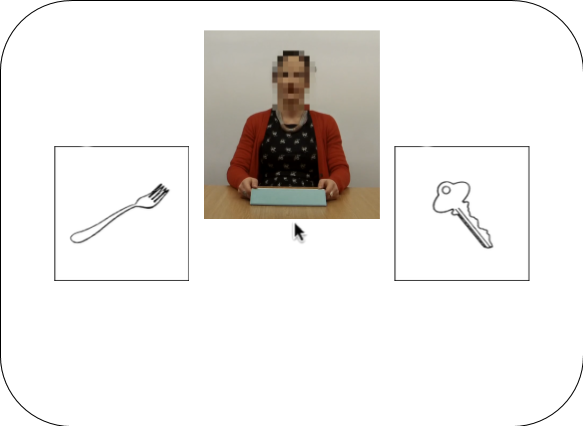
\includegraphics[width=\linewidth]{./img/e7_layout.png}
  \caption{Visual world with video stimulus}
  \label{fig:v1_layout}
\end{figure}

In Experiment~1, we focus on how trunk movements (postural shifts) influence judgements of deception, with filler trials presenting two further types of nonverbal behaviour (adaptor gesturing, and different static postures).
Our focus on trunk movements is based on previous research indicating that listeners perceive these movements as cues to lying \citep{Vrij1996a, Zuckerman1981}.
Trunk movements are also a plausible  utterance-initial gesture, allowing us to ensure that gestures can be viewed in their entirety before visual targets appear and are referred to.  \todo{Jo please check this is accurate}
Based on a post-hoc analysis of filler trials which suggested that listeners' judgements were in fact most strongly influenced by the speaker's adaptor gestures, we designed Experiment~2 to replicate this effect.

\section{Experiment~1}
Experiment~1 makes use of eye  and mouse tracking to investigate whether a speaker's nonverbal behaviours affect a listener's judgements of deception over time. 
The experiment was presented as a `lie detection game'.
Each trial included a video and audio recording of a potentially deceptive speaker describing the location of some hidden treasure.
Throughout a trial, two images, depicting potential treasure locations, remained visible on the screen. 
Participants were tasked with using the mouse to click on the object they believed to be concealing the treasure.
Critical trials presented videos of the speaker either producing a trunk movement immediately prior to utterance playback, or sitting motionless (no cue) for the equivalent amount of time.
Filler trials presented videos of the speaker producing no cue, sitting in a different posture, or producing an adaptor gesture. 
Our aim was to investigate whether and when gestural cues would be associated with falsehood.
%% (add) Our results show that...

\subsection{Participants}
Twenty-four self-reported native speakers of English were recruited from the University of Edinburgh community, and took part in the experiment in return for a payment of \pounds{}4.
Participants all had normal or corrected-to-normal vision, and were all right-handed mouse users.

\subsection{Materials}
Visual stimuli consisted of the same~120 line drawings from \citet{Snodgrass1980} which were used in \citet{Loy2017}, sixty of which served as the object named as hiding the treasure and the other sixty as distractors.
Referents were randomly paired with distractors and presented across sixty trials (20~critical trials and 40~fillers). 
Following \citet{Loy2017}, critical referents and distractors had been matched for both ease of naming and familiarity.
Each referent was associated with a recording of fluent speech specifying the image as the object that the treasure was hidden behind (``The treasure is behind the <referent>'').
Trials also presented a video of a person who was purported to be the speaker of the utterances. 
Videos showed the person speaking\todo{need to rephrase, if face was pixelated they didn't ``show \ldots{} speaking''?}
and either producing a gestural cue or sitting motionless in a neutral posture.
The face shown in the video was pixelated, to allow different videos to be associated with a given audio recording without providing evidence that the visual and auditory channels were recorded separately.
This allowed us to pair invariant audio with different gestures, ensuring that any differences in listener behaviour observed could be attributed entirely to the visual channel.\todo{rewritten}

% videos to be presented alongside different utterances and maintain the illusion that for each trial the spoken utterance heard was the corresponding audio track captured with the video (and produced by the person in the video).

Thirty-five videos were created to pair with audio stimuli which had been previously recorded.
For each video, a volunteer repeated the phrase \spex{the treasure is behind the object} while performing a given gesture (trunk movement, adaptor gesture, different static posture).
% This ensured that when videos were subsequently edited to pixelate the face, pixel movement loosely patterned with the playback of utterances when presented in the experiment). \todo{I can't work out how 35 becomes 60?}
Videos showed the speaker seated at a table upon which rested a tablet computer (on which the referent, distractor, and treasure were purported to be displayed).

Videos used in the 20~critical trials comprised ten videos showing the speaker producing no cue (sitting motionless with her hands on either side of the tablet computer), and five different videos of trunk movements (each presented in two different critical trials).
%%%MC FIXME
In the 40~filler trials, the videos showing no cue from critical trials were presented in two trials each, and 20 videos of other gestures (10 showing adaptor gesturing, and 10 showing the speaker motionless but in a different posture) were each presented in one trial.
Over the course of the experiment each participant saw 30 videos of the speaker producing no cue, and 30 videos of the speaker producing a potential cue to deception (10 showing trunk movements; 10 showing adaptor gestures; 10 showing different postures).

We identified a timepoint in each video at which, according to our judgement, it would be natural for audio to begin. 
For videos showing a trunk movement, this was the frame of the video at which the movement ended, meaning that participants were presented with no overlap between the movement and speech.
These were matched in videos showing no cue, thus controlling for any sensitivity to the duration of video prior to speech (which could be interpreted as speech-initiation time, in turn a potential cue to deception). 
For videos showing an adaptor gesture the amount of overlap between the visual cue and speech varied, and was matched in videos showing the speaker in different static postures.

As with \citet{Loy2017}, 20 critical referents were counterbalanced across two lists. 
Each list contained 10 trials showing a trunk movement video and 10 trials showing a video showing no cue.
The remaining 40 referents were randomly paired with one of the remaining videos (10 showing adaptor gestures, 10 showing different postures, 20 showing no cue) for each participant, with no repetition of referents across videos.

\subsection{Procedure}
The experiment was presented using OpenSesame version~3.1 \citep{Mathot2012}.
Stimuli were displayed on a 21~in.\@ CRT monitor with a resolution of 1024~$\times$~768, placed 850~mm from an Eyelink~1000 Tower-mounted eye tracker which tracked eye movements at 500~Hz (right eye only). 
Audio was sampled at 44100~Hz and presented in stereo from speakers on either side of the monitor. 
Videos were presented at 25~fps, and mouse coordinates were sampled at every frame (every 40~ms).
Eye movements, mouse coordinates and object clicked (referent or distractor) were recorded for each trial.

Figure \ref{fig:v1_trial} represents a sample trial from the experiment. 
Between trials, participants underwent a manual drift correction to ensure accurate recordings from the eye tracker.
After this the central fixation dot turned red for 500ms to signify progression to the trial. 
This was replaced by two images corresponding to the referent and distractor, each measuring 150~$\times$~150 pixels, centered vertically and positioned such that the center of each object was 15\% from either edge of the display. 
The relative positions (left vs.\@ right) of referents and distractors was randomly chosen, with the constraint that each participant saw the referent in an equal number of critical and filler trials on the left as on the right.
This display of two images lasted for 2000~ms before the video was added and the cursor was centred and made visible.
The video, measuring 266~$\times$~284 pixels, was displayed with the bottom edge at the vertical midpoint of the screen and centered horizontally.
Playback of the utterance began at the assigned frame of the video.
The trial ended once the participant clicked on either object, or timed-out 5000~ms after onset of the referent noun, at which point participants saw a message telling them to click on an object faster.

\begin{figure}[Ht]
  \centering
	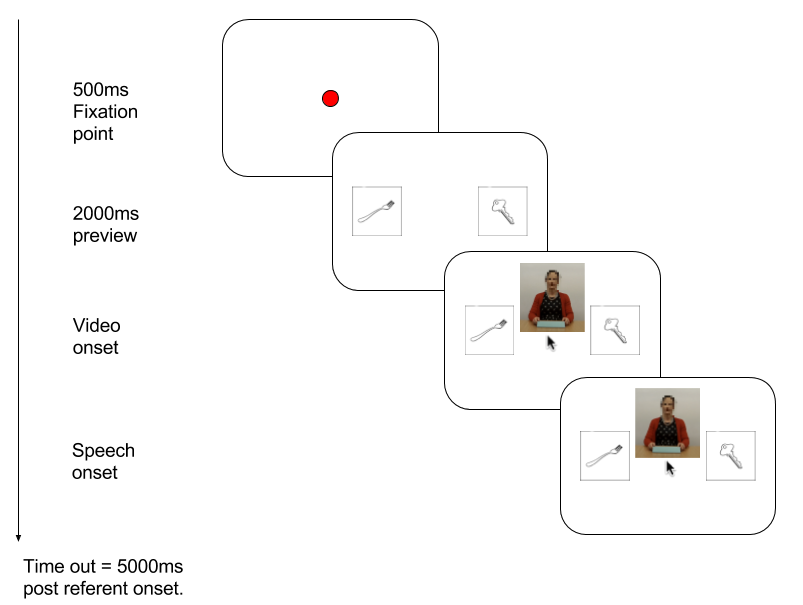
\includegraphics[width=\linewidth]{./img/e7_trial.png}
  \caption{Procedure of a given trial, Experiment~1}
  \label{fig:v1_trial}
\end{figure}

Participants were told that the videos they saw were recordings taken from a previous experiment, in which one participant was tasked with describing the location of some hidden treasure with the aim of misleading the other participant into choosing the wrong location.
To emphasise this, participants were shown a staged photograph of two people purportedly participating in this previous experiment. 
Participants were told that the speakers in the previous experiment had lied approximately half of the time. 
Participants were instructed to click on the object behind which \textit{they believed} the treasure to be hidden, with the overall aim of accumulating as much treasure as they could across the experiment.
Participants received no feedback after their object clicks, except on bonus trials, which are described in the next section.

The order of trials was randomly assigned on each run of the experiment.
Participants completed five practice trials (one of which was presented as a bonus round) prior to the main experiment. 
Two of these presented a video showing no cue, two displayed a video of the speaker in different postures, and one displayed a video of the speaker making a trunk movement.


\subsection{Bonus Trials}
To maintain motivation throughout the study, participants were told that there were a number of ``hidden bonus rounds'' which offered more treasure than regular rounds.
25\% of filler trials (half presenting a video showing either adaptor gesturing or a different posture; half presenting a video showing no cue) were randomly designated as bonus rounds for each participant.
These trials were visually identical to regular trials.
However, following the mouse click (regardless of the object chosen), a message was displayed informing participants that they had successfully located bonus treasure.
Participants were told that the top scorers would be able to enter their names on a high-score table, which was shown at the beginning of the experiment. 

\subsection{Post-test Questionnaire}
Participants were asked to complete a short post-test questionnaire which asked whether participants had noticed anything odd about the visual or audio stimuli.
Any participant who indicated that they had noticed anything unusual was then questioned further, to decide whether they believed that the speech and gesture had been produced naturally and simultaneously.
All participants were subsequently debriefed, during which they were told that the audio and video were created separately and stitched together, and asked again verbally if they noticed anything unusual in that respect. 
Responses to the questionnaire and debrief were used to determine whether participants should be excluded from the analysis.

\section{Results}

\subsection{Analysis}
Analysis of critical trials was carried out in R version~3.4.4 \citep{Rbase2017}, using the lme4 package version~1.1-17 \citep{Bates2015}. 
Data from four participants who indicated suspicion of the supposed origins of the audiovisual stimuli based on the post-test questionnaire and/or debrief were removed from all analyses, leaving data from twenty participants. 
Of 400 critical trials, one trial in which participants did not click on either the referent or distractor was excluded from all analyses.

Object clicked (referent or distractor) was modelled using mixed effects logistic regression, with a fixed effect of nonverbal behaviour in the video (no cue vs.\@ trunk movement, dummy coded with no cue as the reference), with random intercepts and slopes for nonverbal behaviour both by-participant and by-item.
Reaction times (measured from referent onset) were log transformed and modelled with the same fixed and random effect structure using mixed effects linear regression.

Eye fixation data was averaged into 20~ms bins (of 10 samples) prior to analysis.
For each bin, we calculated the proportions of time spent fixating the referent or the distractor, resulting in a measure of the proportions of fixations on either object over time.
The position of the mouse was sampled every 40~ms.
Using the $X$ coordinates only, we calculated the number of screen pixels moved and the direction of movement (towards either referent or distractor).
We then calculated the cumulative distance travelled towards each object over time as a proportion of the cumulative distance travelled in both directions from referent onset up until that time bin.
Movements beyond the outer edge of either object were considered to be `overshooting' and were not included in calculations (0.8\% of samples).
Eye  and mouse  biases were calculated from the proportions of referent to distractor fixations, and were subsequently empirical logit transformed \citep{Barr2008}. 
In these measures, a value of zero indicates no bias towards either object, and positive and negative values indicate a bias towards the referent and distractor respectively.

As in previous studies using the treasure game paradigm \citep{King2018,Loy2017}, eye  and mouse  tracking analyses were conducted on a time-window beginning at referent onset and extending for 800~ms, just beyond the duration of the longest critical referent (776~ms).
Eye and mouse data was modelled over this time window using linear mixed effects models, with fixed effects of time from referent onset (seconds), nonverbal behaviour (dummy coded with no cue as reference level), and their interaction.
Random intercepts and slopes for time and nonverbal behaviour were included both by-item and by-participant.
Following \citet{Baayen2008}, we considered effects in these models to be significant where $|t|>2$.

\subsection{Object clicks}
Participants clicked on the referent in 56\% of critical trials and the distractor in 44\%.
Table \ref{table:v1_clicks} shows the percentage of clicks across all participants to either object split by whether the video showed no cue or a trunk movement.
Participants were more likely to click on the referent than the distractor following a video showing no cue. 
This was a marginal reduction of this bias following videos of the speaker producing a trunk movement (\resultsLog{-0.56}{0.32}{=0.08}).
There was no effect of nonverbal behaviour on the time taken by participants to click on an object.


\begin{table}
\caption{Breakdown of mouse clicks recorded on each object (referent or distractor) by condition in critical trials in Experiment~1}
\label{table:v1_clicks}
\begin{tabularx}{\linewidth}{YYYYY}
\hline
& No Cue & Trunk Movement \\
Clicks to Referent & 125 (62.5\%) & 99 (49.7\%) \\ 
Clicks to Distractor & 75 (37.5\%) & 100 (50.3\%) \\
\hline
\end{tabularx}
\end{table}

\subsection{Eye movements}
Figure \ref{fig:v1_eye1} shows the time course of fixations to referents and distractors in critical trials for the 2000~ms from referent onset, split by the type of nonverbal behaviour presented in the video. \todo{JK > MC: I can't seem to word these results in a way that is intuitive to you. See .tex for fixef, and if you can give an example of what wording would be most clear, then that would be great.}
Analysis conducted over the 800~ms period from referent onset showed that, following videos showing no cue to deception, participants became increasingly likely to fixate the referent over the distractor as this window progressed (as indicated by a main effect of time \resultsLM{2.23}{0.67}{=3.34}).
Importantly, there was no interaction of time with nonverbal behaviour, indicating that the presence of trunk movements did not influence participants' increasing fixation bias toward the referent. 

%remember that time is not centered
%                              Estimate Std. Error t value
%(Intercept)                    -0.3833     0.3157  -1.214
%vid_typeTrunk Movement         -0.1754     0.3260  -0.538
%time_s                          2.2311     0.6675   3.342
%vid_typeTrunk Movement:time_s   0.3448     0.2236   1.542


\begin{figure}[Ht]
  \centering
	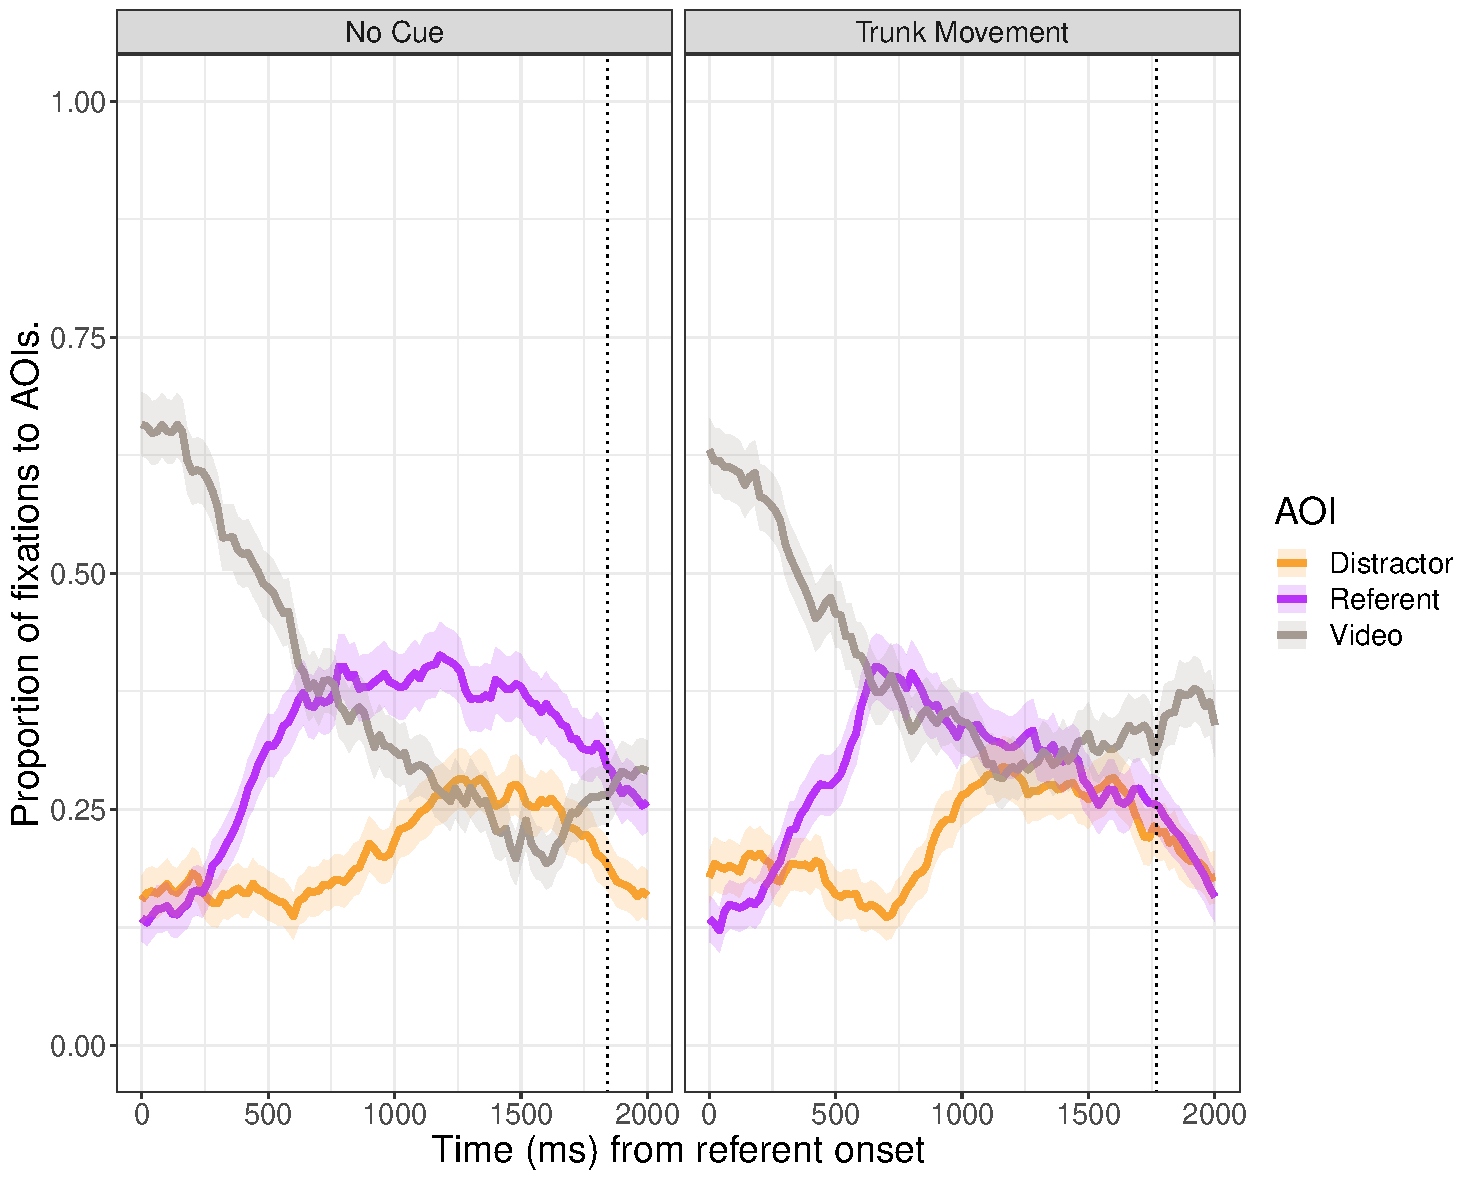
\includegraphics[width=\linewidth]{./img/e7_fixations_crit.pdf}
  \caption{eye tracking results for critical trials in Experiment~1: Proportion of fixations to each object (referent or distractor) and the video, from 0 to 2000 ms post-referent onset, calculated out of the total sum of fixations for each 20~ms time bin. Shaded areas represent $\pm$ 1 standard error of the mean.}
  \label{fig:v1_eye1}
\end{figure}

\subsection{Mouse movements}
Figure \ref{fig:v1_mouse1} shows the time course of the proportions of cumulative distance the mouse moved towards the referent and distractor in critical trials for the 2000~ms period from referent onset, split by whether the video showed either no cue or a trunk movement.
Analysis on the 800~ms following referent onset showed that participants' mouse movements patterned with their eye movements:
Over the course of the window participants were increasingly likely to have moved more towards the referent than the distractor following videos of no cue (\resultsLM{0.30}{0.12}{=2.41}). 
Videos showing the speaker producing a trunk movement did not influence this increasing referent bias.


\begin{figure}[Ht]
  \centering
	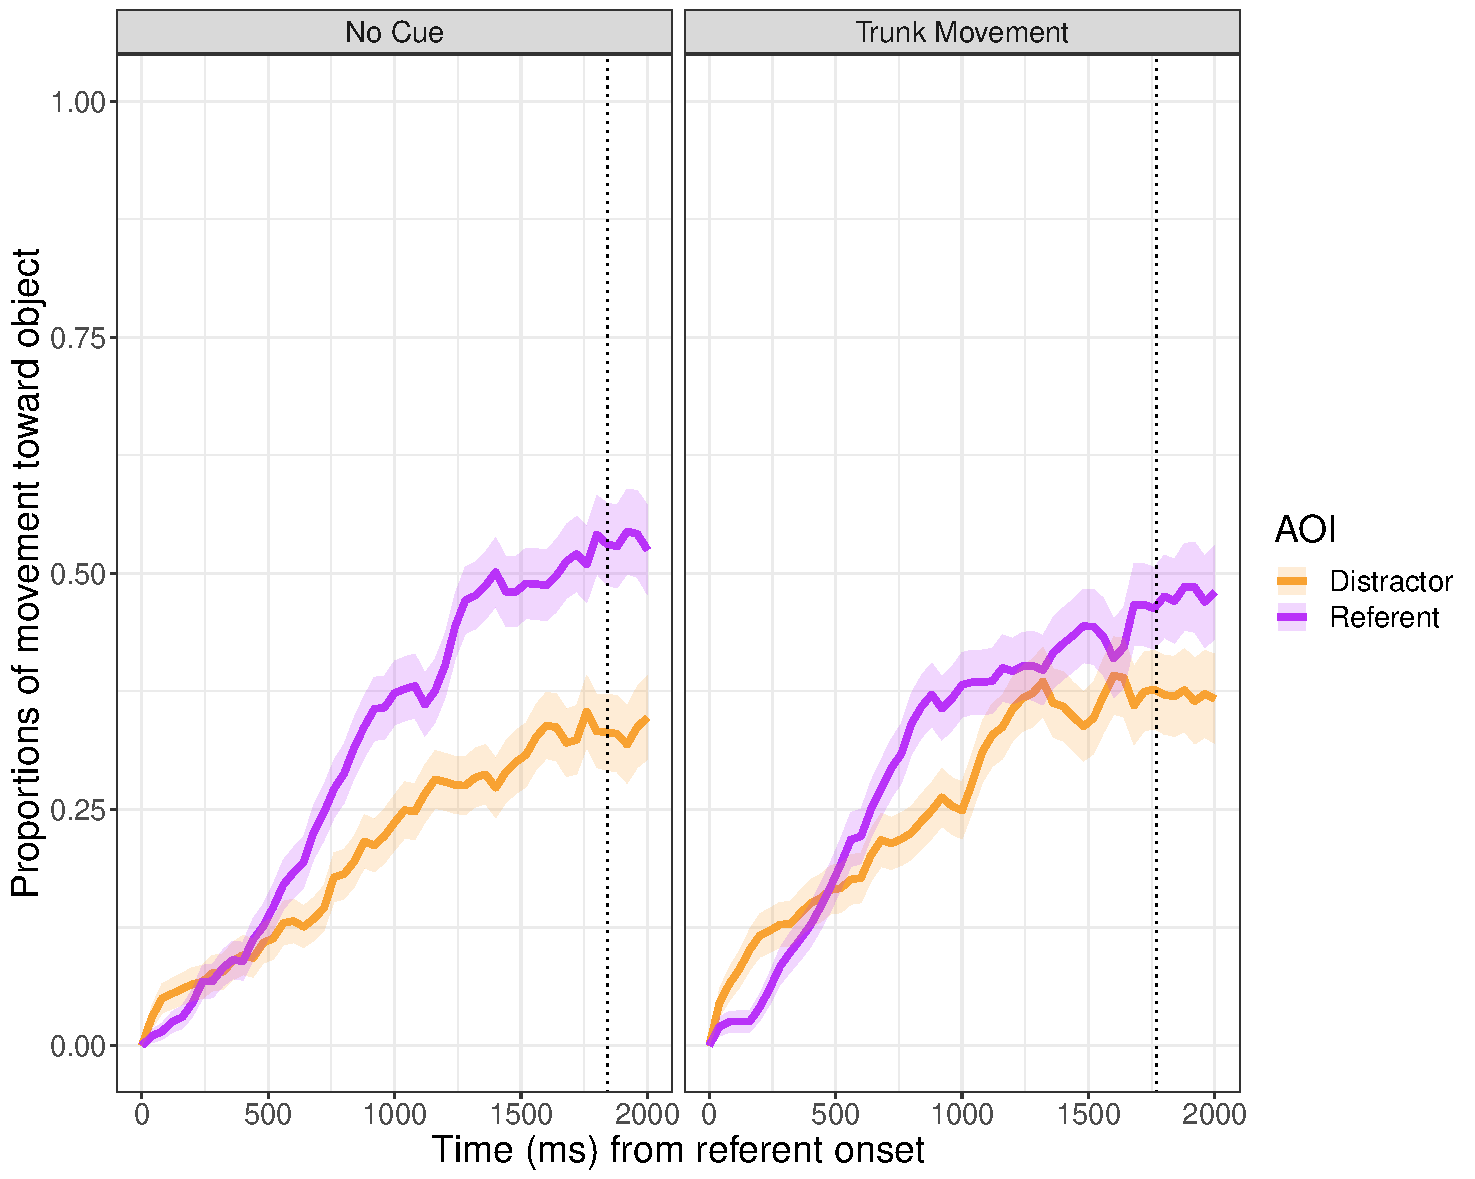
\includegraphics[width=\linewidth]{./img/e7_mouse_crit.pdf}
  \caption{mouse tracking results for critical trials in Experiment~1: Proportion of cumulative distance traveled toward each object from 0 to 2000 ms post-referent onset. Proportions were calculated from the total cumulative distance participants moved the mouse until that time bin. Shaded areas represent $\pm$ 1 standard error of the mean.}
  \label{fig:v1_mouse1}
\end{figure}

\section{Additional Analyses of Filler trials}
In the post-test verbal questioning, 8 (40\%) of participants specifically mentioned responding to the speaker's hand-movements in their judgements of whether or not the speaker was deceptive. 
We conducted analyses on filler trials to investigate whether the types of nonverbal behaviours presented in these trials (different postures and adaptor gesturing) were influencing participants' judgements of deception.
Analysis of filler trials was conducted on 797 trials (3 trials were excluded from analysis due to no mouse click on either object), with nonverbal behaviour comprising three levels: No cue, different posture and adaptor gesture. %% jia: mention - no cue again reference level?
The time-window of analysis for eye  and mouse  movements was extended to 1100~ms to include the duration of the longest referent in filler trials (1062~ms).
Model specification was the same as for analysis of critical trials, with the exception of the removal of all by-item random effects of nonverbal behaviour (this was necessary as videos in filler trials were not counterbalanced across items).

\subsection{Object clicks}
Table \ref{table:v1_filler_clicks} shows the percentage of clicks in filler trials across all participants to either object, split by the type of nonverbal behaviour presented in the video.
Results show that for trials in which the video showed a speaker producing no cue, participants tended to click on the referent rather than the distractor (\resultsLog{0.63}{0.16}{<0.001}).
For trials in which the videos showed the speaker either in a different posture and or producing an adaptor gesture, this bias to click on the referent was reduced (\resultsLog{-0.73}{0.31}{=0.02}) and \resultsLog{-1.03}{0.33}{=0.002} respectively), suggesting that presence of these types of nonverbal behaviour influenced participants' final judgements of whether the speaker was truthful or dishonest.


\begin{table}
\caption{Breakdown of mouse clicks recorded on each object (referent or distractor) for each type of nonverbal behaviour presented in the filler trials for Experiment~1}
\label{table:v1_filler_clicks}
\begin{tabularx}{\linewidth}{YYYYY}
\hline
& No-Cue & Different Posture & Adaptor Gesture \\
Clicks to Referent & 256 (64.5\%) & 96 (48.0\%) & 83 (41.5\%) \\ 
Clicks to Distractor & 141 (35.5\%) & 104 (52.0\%) & 117 (58.5\%) \\
\hline
\end{tabularx}
\end{table}

\subsection{Eye movements}
Figure \ref{fig:v1_eye2} shows the time course of proportions of fixations to referent and distractor split by the type of nonverbal behaviour shown in the filler trials. 
Analysis conducted on the 1100~ms following referent onset revealed that, as in critical trials which showed the speaker producing no obvious cue to deception, participants tended to fixate the referent over the distractor more as time increased (\resultsLM{1.05}{0.34}{=3.13}). 
However, this bias towards the referent over time was attenuated following both videos showing the speaker in a different posture and those in which the speaker was shown to produce an adaptor gesture (\resultsLM{-0.58}{0.13}{=-4.42} and \resultsLM{-0.96}{0.13}{=-7.31} respectively).

%(Intercept)                        0.1708     0.2214   0.771
%vid_typeAdaptor Gesture           -0.1298     0.2378  -0.546
%vid_typeDifferent Posture          0.2510     0.2274   1.104
%time_s                             1.0512     0.3363   3.126
%vid_typeAdaptor Gesture:time_s    -0.5810     0.1316  -4.417
%vid_typeDifferent Posture:time_s  -0.9641     0.1319  -7.307

\begin{figure}[Ht]
  \centering
	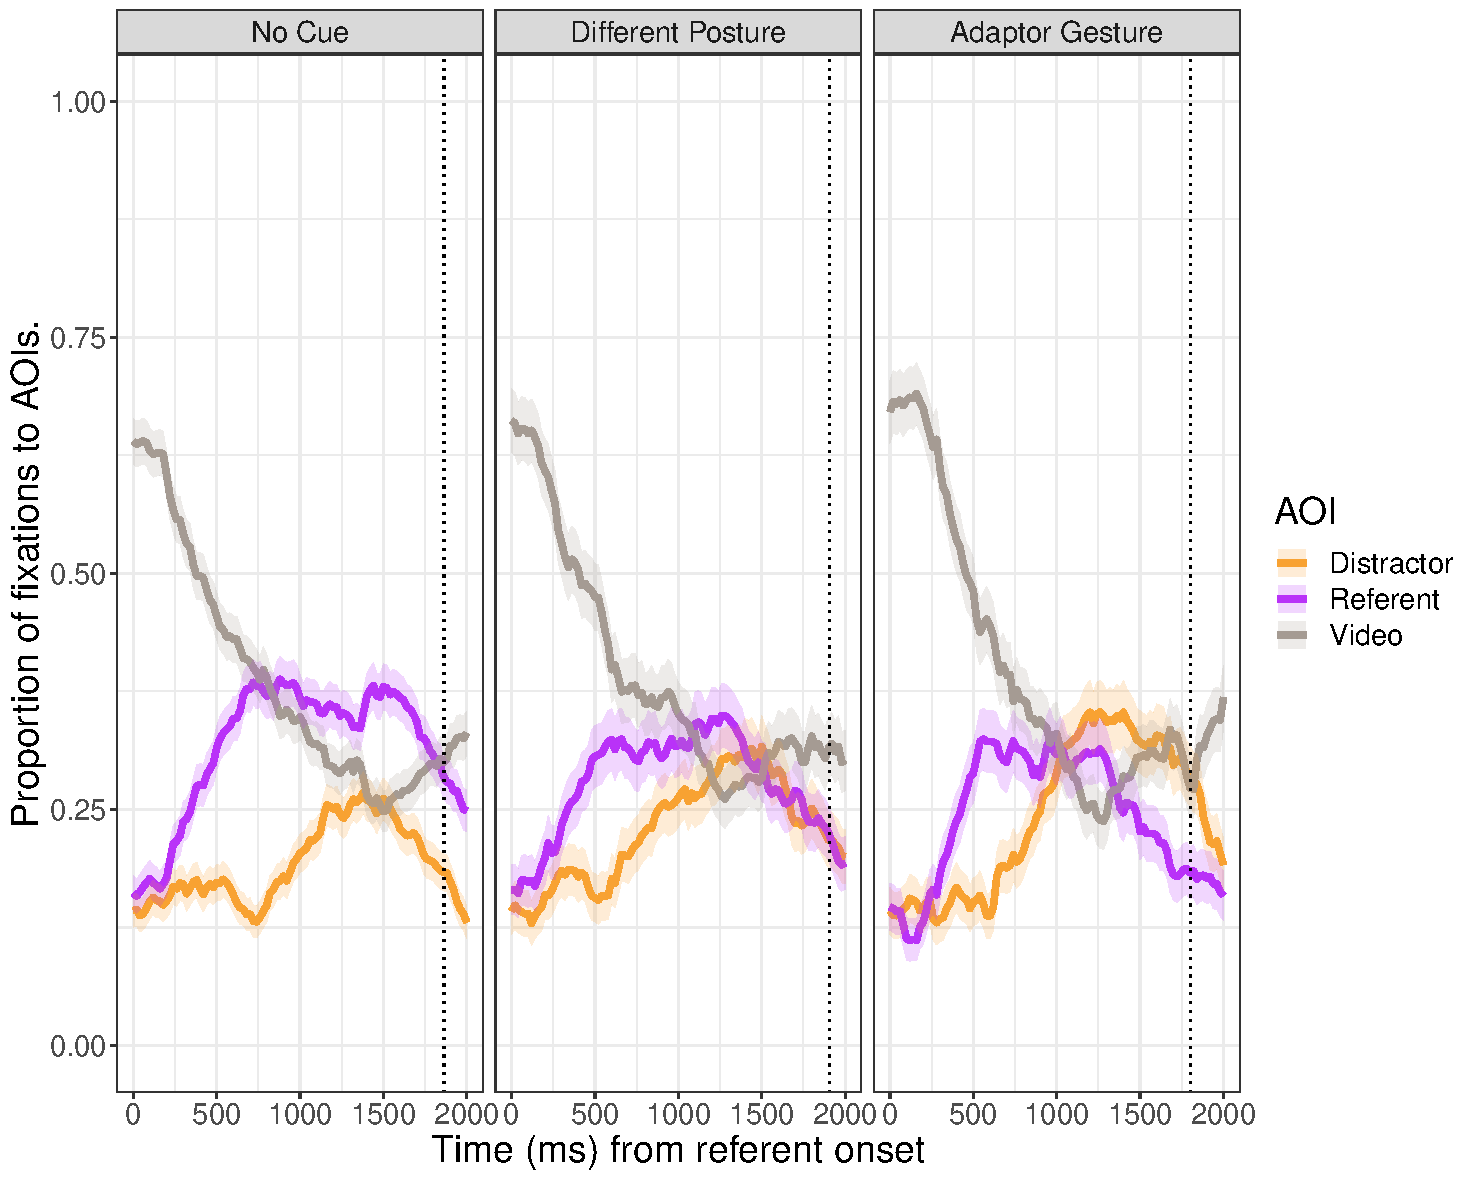
\includegraphics[width=\linewidth]{./img/e7_fixations_filler.pdf}
  \caption{eye tracking results for filler trials in Experiment~1: Proportion of fixations to each object (referent or distractor) and the video, from 0 to 2000 ms post-referent onset, calculated out of the total sum of fixations for each 20~ms time bin. Shaded areas represent $\pm$ 1 standard error of the mean.}
  \label{fig:v1_eye2}
\end{figure}

\subsection{Mouse movements}
Figure \ref{fig:v1_mouse2} shows participants' mouse movements towards the referent and distractor split by the type of nonverbal cue shown in the filler trials. 
Analysis conducted on the 1100~ms following referent onset showed that mouse movements patterned with eye movements.
The increasing bias over time to move towards the referent rather than the distractor following videos in which the speaker produced no cue (\resultsLM{0.40}{0.08}{=4.71}) was reduced following videos showing the speaker in a different posture (\resultsLM{-0.22}{0.05}{=-4.41}) and producing an adaptor gesture (\resultsLM{-0.35}{0.05}{=-7.19}).

\begin{figure}[Ht]
  \centering
	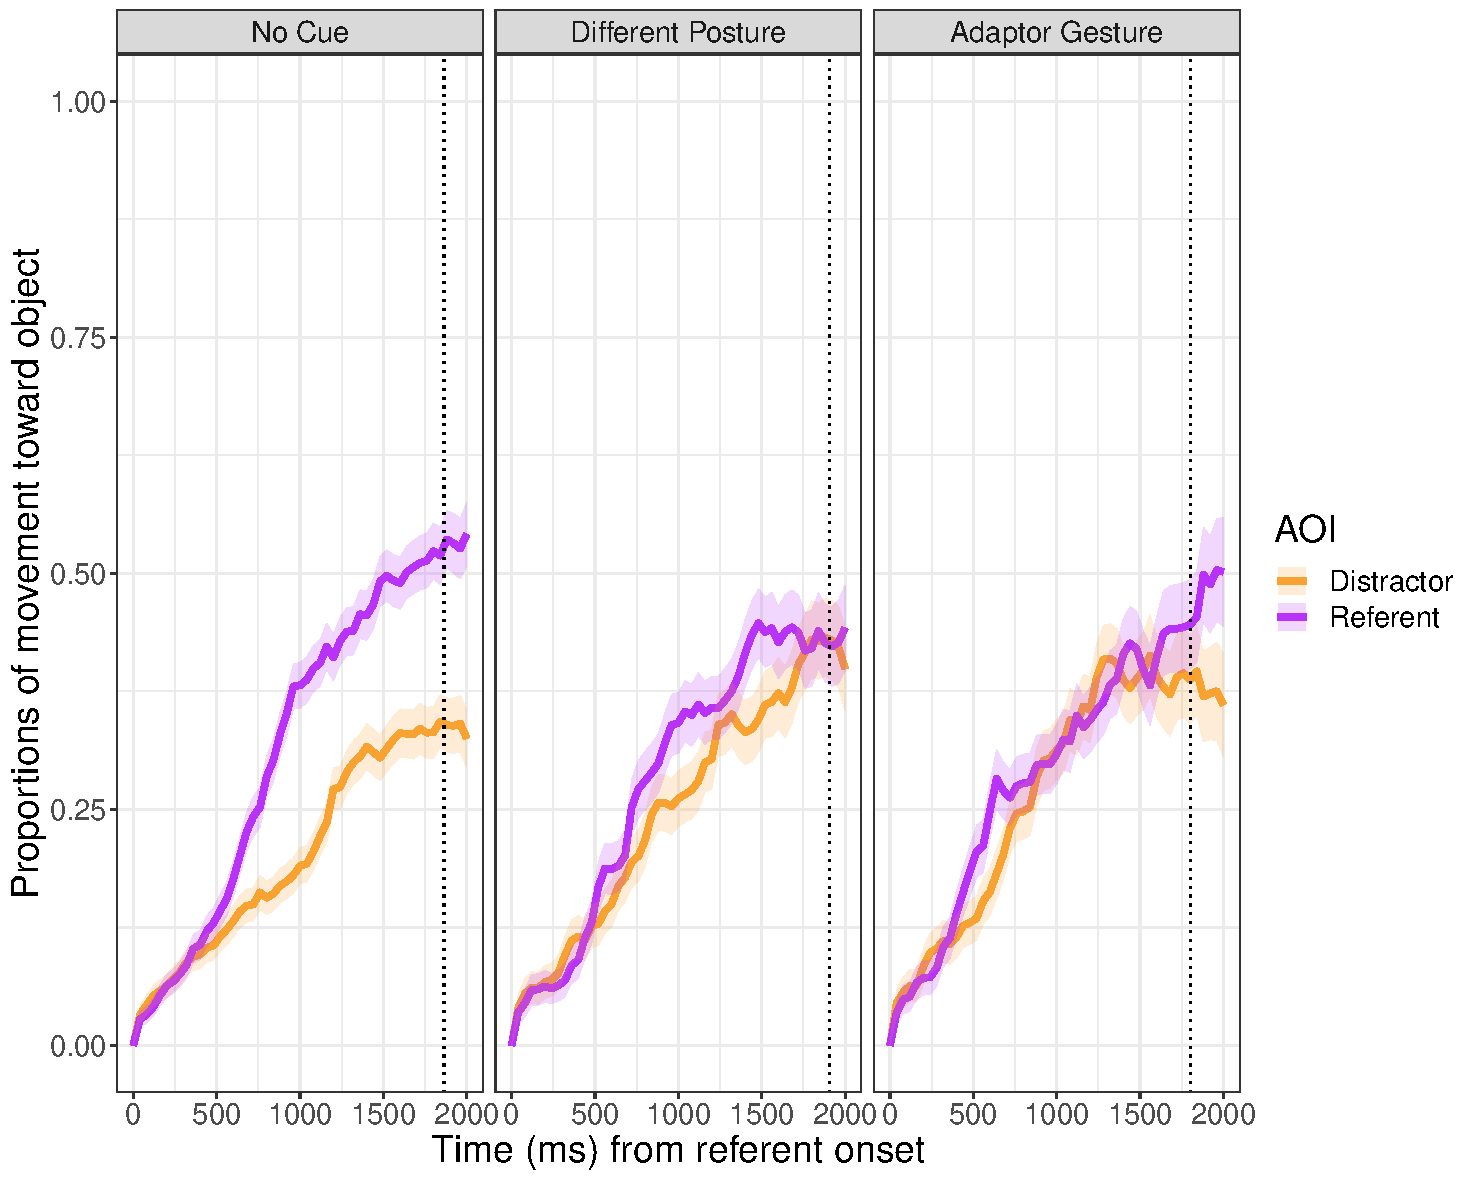
\includegraphics[width=\linewidth]{./img/e7_mouse_filler.pdf}
  \caption{mouse tracking results for filler trials in Experiment~1: Proportion of cumulative distance traveled toward each object from 0 to 2000 ms post-referent onset. Proportions were calculated from the total cumulative distance participants moved the mouse until that time bin. Shaded areas represent $\pm$ 1 standard error of the mean.}
  \label{fig:v1_mouse2}
\end{figure}

\section{Discussion}
Experiment~1 investigated how the pragmatic inferences listeners make about a speaker's honesty are influenced by presence of nonverbal cues to deception in the form of trunk movements.
We measured eye  and mouse  movements of participants who were presented with a task in which they made decisions about the true location of some treasure based on audio and video of a potentially deceptive speaker making a statement about the treasure's location.
Participants were thus making implicit decisions about the honesty of each utterance.
As in previous studies using versions of this paradigm \citep{Loy2017, King2018}, participants showed a tendency to interpret an utterance as truthful (as indicated by more clicks to the named object) when there was no obvious cue to deception (i.e. speaking fluently, or sitting motionless).
The presence of trunk movements in the videos which were presented alongside utterances had only a marginal influence on participants' judgements of deception based on their final object clicks.
Participants' eye  and mouse  movements during the 800~ms following referent-onset were likewise not affected by whether the video showed the speaker producing a trunk movement or no cue.

Additional analyses of filler trials suggested that participants' may have been basing their judgements on the other types of nonverbal behaviour presented in these trials---videos showing the speaker producing either an adaptor gesture or sitting in a different posture were associated with more judgements of deception than videos showing the speaker producing no cue.
Furthermore, the influence of these nonverbal cues was evident in the early stages of reference comprehension, as indicated by a weakening of the bias to fixate and move towards the referent over the distractor. 
However, it is possible that the effects observed in filler trials were due to analysis over an extended time window of analysis (extended due to longer referents), making it difficult to draw comparisons to previous research in to spoken cues to deception. 

Counter to our prediction that trunk movements would be associated with lying, these findings suggest that listeners may in fact rely on other visual cues when making judgements of deception.
One possible explanation for why participants did not reliably associate trunk movements with deception could be that utterance-initial nonverbal cues may not be interpreted similarly to utterance-initial speech cues in the context of judging deception.
Evidence points to the integration of illustrative gesturing with speech being tightly linked to their temporal synchrony \citep[See][]{Habets2011}, something which may also apply to the types of gesturing included here.
This would explain why disfluencies both preceding and during utterances were associated with judgements of deception in \citet{Loy2017}, but the utterance-initial trunk movements in our study were not.

Overall, results from Experiment~1 contrast with previous findings in the literature which suggest that listeners strongly associate trunk movements with lying \citep[e.g.][]{Vrij1996a, Zuckerman1981}.
Analysis of filler trials indicates that participants may have been associating deception more with adaptor gestures and different static postures. 
From a practical viewpoint, the time course of participants' eye  and mouse movements in Experiment~1 support the compatibility of the visual world paradigm with a range of video stimuli: Even when viewing videos in which movements co-occurred with speech (e.g. adaptor gestures), visualisation of proportions of fixations indicate that the video did not prevent a fixation bias evident in the early stages of reference comprehension.
Furthermore, small movements such as finger tappings appeared to be salient enough to influence participants' final judgements of deception.
However, the nonverbal behaviours that appeared to  have the greatest influence on participants' judgements were never the intended focus of Experiment~1, and these trials differed from critical trials in a number respects (counterbalancing of videos across referents, and the possibility of `hidden bonus round' feedback).
We therefore designed Experiment~2 as a more controlled investigation of the association between adaptor gesturing and perceived dishonesty.
Participants in Experiment~2 saw videos of a speaker either producing an adaptor gesture, or sitting motionless, and there were no filler trials.

\section{Experiment~2}
Using the same paradigm as Experiment~1, participants in Experiment~2 heard utterances accompanied by a video of a speaker either producing an adaptor gesture or sitting motionless, and were tasked with making an implicit judgement on whether the speaker was lying or telling the truth.
Videos in Experiment~2 showed adaptor gestures which have previously suggested to be associated with nervousness \citep[See][]{Gregersen2005}, and videos were pre-tested for perceived anxiety in the speaker.
As a manipulation check, after the treasure-game task, participants were asked to rate how nervous the speaker looked in each video (without audio).

\subsection{Participants}
Twenty-three self-reporting native English speaking participants took part in exchange for \pounds{}3 compensation.

\subsection{Materials}
The 40 images used in critical trials in Experiment~1 (20 referents; 20 distractors) were used across twenty trials.
As in Experiment~1, these images were displayed in referent-distractor pairs, with each pair shown alongside a recorded utterance naming the referent as the location of the treasure.
The pairing of referents and distractors on each trial was randomised.

As in Experiment~1, each pair of images and recorded utterance was presented alongside a video clip of a person purported to be the speaker of the utterance.
Twenty-eight new video clips were recorded (18 different adaptor gestures; 10 no-cue). 
Care was taken to ensure that the videos including no cue showed the speaker in a relaxed posture. 
Adaptor gestures were based on descriptions of anxious nonverbal behaviour from \citet{Gregersen2005}.
All 28 videos were pre-tested for perceived nervousness of the speaker.
Ten native english speakers were told that they were going to watch videos (without audio) of someone being questioned in a stressful situation, and were asked to rate how nervous the speaker looked in each video (1: very relaxed, 7: very nervous). 
The 10 videos showing adaptor gestures with the highest ratings (Mean = 4.1, SD = 1.5) were included in the experiment, along with the 10 videos showing no cue (Mean = 1.9, SD = 1.1).

The 20 referents were counterbalanced across two lists such that each referent that occurred with a video showing adaptor gesturing in the first list occurred with a video showing no cue in the second.
The pairings of referents with specific videos within each condition was randomised on each run of the experiment.

\subsection{Procedure}
The experiment procedure was identical to that of Experiment~1 with the following changes.
First, the size of the video stimuli changed slightly, and measured 236~$\times$~336 pixels.
Second, the duration of video presented prior to audio playback was set at a fixed constant (1400~ms).
Third, we did not include any `bonus' trials, so participants did not receive any feedback during the experiment.

After the main task, participants were asked to watch all 20 videos again, without audio, and asked to rate how nervous they thought the speaker looked (using the same 1-7 scale as described above).
Participants then completed the same post-test questionnaire as in Experiment~1, with data being excluded from analysis on the same basis.

\section{Results}
Data from three participants were excluded due to suspicion of the audiovisual stimuli being scripted (based on the post-test questionnaire and questioning during debrief), and analysis was conducted on data from the remaining 20 participants.

\subsection{Analysis}
We followed the same analysis strategy as was used for the critical trials in Experiment~1.
Of the 400 trials, those which did not result in a click to either object (3) were excluded from analyses.
Analyses was identical to that of the critical trials in Experiment~1.

\subsection{Object clicks}
Across the experiment, participants clicked on the referent in 53\% of trials and the distractor in the remaining 47\%.
Table \ref{table:v2_clicks} shows the proportions of clicks to either object for each type of nonverbal behaviour presented in the videos (no cue vs.\@ adaptor gesturing).
As in Experiment~1, following videos showing the speaker sitting motionless, participants were more likely to click on the referent than the distractor (\resultsLog{1.53}{0.23}{<0.001}).
The nonverbal behaviour of the speaker in the video was found to influence participants' judgements of deception: 
Relative to videos showing no cue to deception, those showing adaptor gesturing in the video resulted in fewer clicks to the referent (\resultsLog{-2.78}{0.38}{<0.001}).
The time participants took to click on an object was not influenced by the behaviour shown in the video.

\begin{table}
\caption{Breakdown of mouse clicks recorded on each object (referent or distractor) by condition in Experiment~2}
\label{table:v2_clicks}
\begin{tabularx}{\linewidth}{YYY}
\hline
& No Cue & Adaptor gesture \\
Clicks to Referent & 161 (80.9\%) & 48 (24.2\%)  \\
Clicks to Distractor & 38 (19.1\%) & 150 (75.8\%)  \\
\hline
\end{tabularx}
\end{table}

\subsection{Eye movements}
Figure \ref{fig:v2_eye} shows the time course of fixations to referents and distractors over 2000~ms from referent onset, split by condition.
Analyses conducted over the time window of 800~ms post-referent onset revealed a main effect of time (\resultsLM{2.99}{0.67}{=4.48}), indicating that, as in Experiment~1, participants tended to fixate the referent over the distractor more as this window progressed.
However, a significant interaction between time and the nonverbal behaviour presented in the video (\resultsLM{-2.94}{0.21}{=-14.27}) indicates that the increasing referent-bias was attenuated in trials showing the speaker producing an adaptor gesture. 

\begin{figure}[Ht]
  \centering
	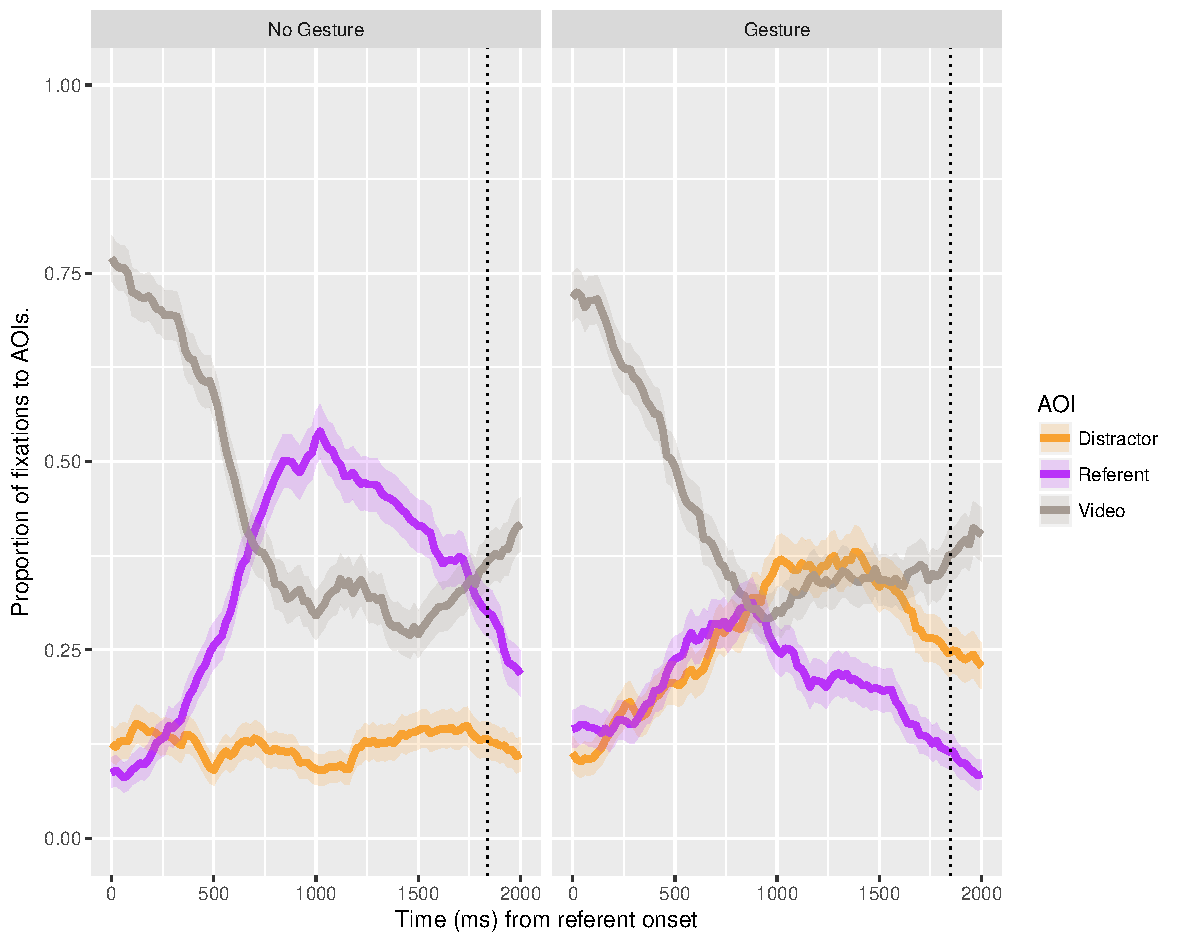
\includegraphics[width=\linewidth]{./img/e8_fixations.pdf}
  \caption{eye tracking results for Experiment~2: Proportion of fixations to each object (referent or distractor) and the video, from 0 to 2000 ms post-referent onset, calculated out of the total sum of fixations for each 20~ms time bin. Shaded areas represent $\pm$ 1 standard error of the mean.}
  \label{fig:v2_eye}
\end{figure}

\subsection{Mouse movements}
Figure \ref{fig:v2_mouse} shows the time course of the proportions of cumulative distance the mouse moved towards the referent and distractor for 2000~ms from referent onset, split by condition.
mouse movements over the course of the 800~ms window from referent onset again patterned with the eye tracking data:
As time from referent onset increased, participants showed an increasing likelihood of having moved more toward the referent than the distractor following videos showing the speaker producing no cue (\resultsLM{0.61}{0.10}{=5.88}), but this was reduced following videos showing an adaptor gesture (\resultsLM{-0.78}{0.08}{=-9.27}).


\begin{figure}[Ht]gesture
  \centering
	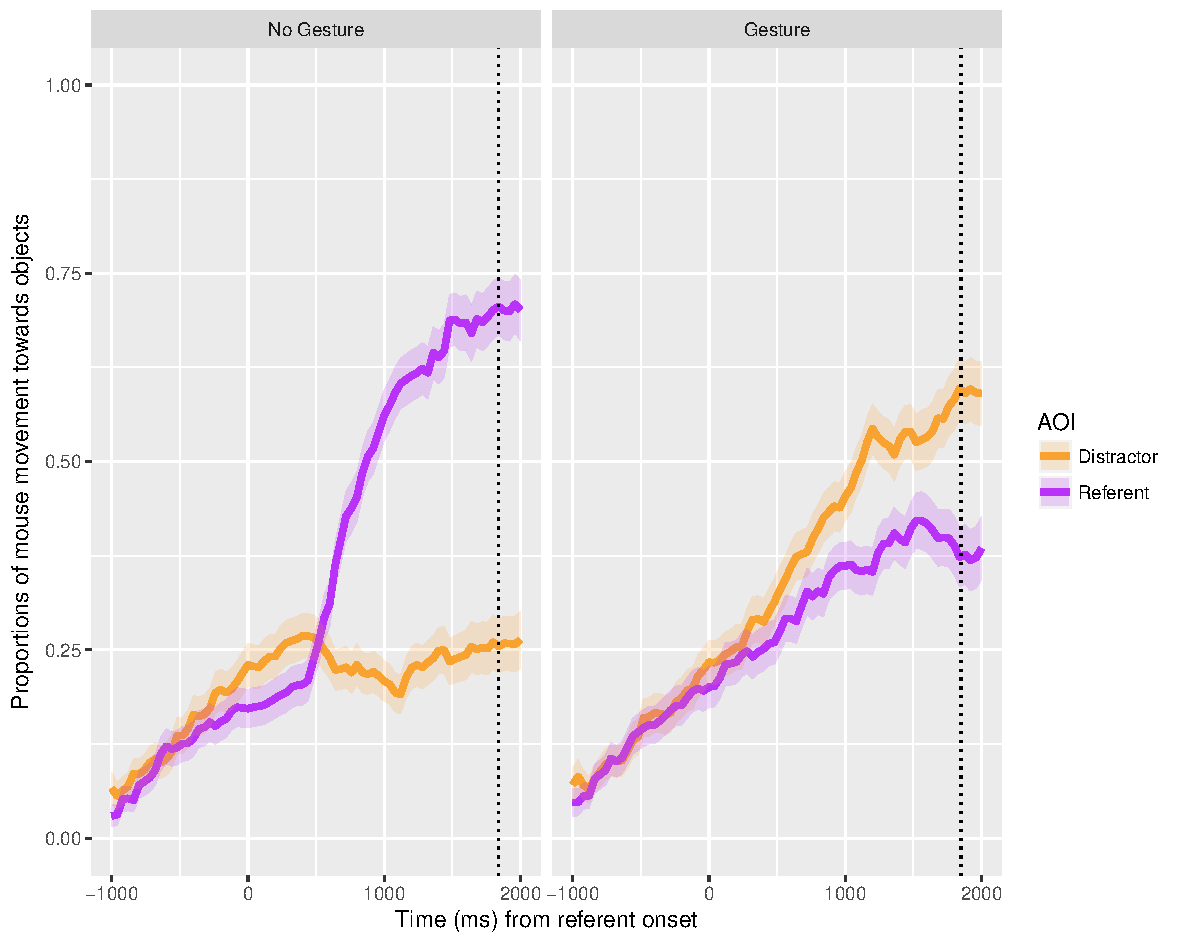
\includegraphics[width=\linewidth]{./img/e8_mouset.pdf}
  \caption{mouse tracking results for Experiment~2: Proportion of cumulative distance traveled toward each object from 0 to 2000 ms post-referent onset. Proportions were calculated from the total cumulative distance participants moved the mouse until that time bin. Shaded areas represent $\pm$ 1 standard error of the mean.}
  \label{fig:v2_mouse}
\end{figure}

\section{General discussion}

Experiments~1 and 2 investigate the integration of a speaker's nonverbal behaviour into judgements of deception, focussing on listeners' associations of trunk movements and adaptor gesturing with deception respectively.
We manipulated the presentation of different potential nonverbal cues to deception while measuring eye and mouse movements of the listener towards one of two possible final judgements about the whether the speaker was honest or dishonest for a given utterance.
This allowed us to explore if, and when, listeners began to associate nonverbal cues with deception.


In Experiment~1, the presence of nonverbal cues in the form of trunk movements were found to have only a marginal effect on listeners' judgements of deception, and did not influence the patterns of eye  and mouse movements in the 800~ms following referent onset, which showed an overall tendency to fixate on and move the mouse towards the referent over the distractor.
The contrast of these findings with previous research \citep[e.g.][]{Vrij1996a} may reflect differences between beliefs about cues to deception (as indicated in questionnaires) and those cues which listeners associated with deception when presented with them.
Alternatively, the inclusion of additional nonverbal behaviours in filler trials may have weakened the association between trunk movements and deception which has been found in previous research \citep[e.g][]{Vrij1996a, Zuckerman1981}.
This is partly supported by studies which found a facilitative effect of illustrative gesturing on listeners' comprehension to be weakened for speakers who produce a lot of other, non-communicative movements \citep{Holle2007}. 

Additional analyses indicated that other types of nonverbal behaviour used in filler trials (different static postures and adaptor gestures) were associated with more judgements that the speaker was being deceptive, and that these associations were evident in the early stages of comprehension (although over a longer window of analysis than previous studies using this paradigm).
Experiment~2 was conducted to further investigate the influence of adaptor gestures on judgements of deception in a study designed specifically to this end.
Using the same paradigm, videos in Experiment~2 showed the speaker either producing an adaptor gesture or sitting motionless, and there were no filler trials. 
Results indicate a reliable association between adaptor gesturing and perceived dishonesty.
Furthermore, the influence of adaptor gesturing on listeners' judgements of deception was present in the early stages of reference comprehension.
Relative to videos showing no cue to deception, participants' tendency to fixate and move the mouse towards the referent (over the distractor) more as time increased was attenuated following videos showing the speaker producing an adaptor gesture.

The studies presented here provide a visual-modality parallel with the findings from \citet{Loy2017} which showed that fluency of speech influences judgements of whether a speaker is lying.
Comparably to \citet{Loy2017}, our results suggest that listeners may have an implicit bias to judge a speaker as honest in the absence of any obvious potential cue to deception.
In both experiments, utterances presented with the speaker in a neutral posture and not gesturing biased listeners towards believing the speaker to be truthful, as shown by increased tendency to fixate on, move the mouse towards, and eventually click on the object which was named by the speaker. 

Similarly to the effect of manner of spoken delivery on these judgements found in \citet{Loy2017}, we found that manner of nonverbal delivery influenced judgements of deception, in particular when the speaker was seen to produce adaptor gesturing alongside speech.
Importantly, this was detectable in the initial stages of linguistic processing, with effects found in Experiment~2 during the same time window as that in which \citet{Loy2017} found effects of speech disfluency.
However, visual inspection of Figure \ref{fig:v2_eye} suggests that when presented with a video showing a speaker producing an adaptor gesture, the bias to fixate the distractor --- signifying perceived dishonesty --- over the referent emerges approximately 1000~ms after the referent began. 
This contrasts with \citet{Loy2017}, in which the bias emerged approximately 600~ms post referent onset following both utterance initial and utterance medial disfluencies. 
Whether this discrepancy suggests a difference in how audio and visual cues are integrated into pragmatic judgements of deception, or whether this is simply a result of the presence of a video in the display delaying the emergence of a fixation bias, we cannot say. 
To better understand how information in different modalities affect comprehension, further research would require investigating the effect of spoken delivery when the visual channel is also available --- for example, studying the time course of deception judgements when faced with one or both of a disfluency and an adaptor gesture.

Our findings are largely consistent with previous research on beliefs about and judgements concerning nonverbal cues to deception, suggesting that listeners perceive a range of nonverbal behaviours to indicate deceit \citep[e.g.][]{Akehurst1996, Vrij2000}.
However, the lack of a reliable association between trunk movements and judgements of deception suggests that care should be taken when generalising from peoples' beliefs about cues to deception \citep[e.g.][]{Vrij1996a, Zuckerman1981} to situations in which they are faced with a variety of possible cues.

It is worth noting that the studies presented here show the possible benefits to be gained in extending the visual world paradigm to include visual information about the speaker, and not just the extensional world. % Jia: what studies?
Our findings show how, by including a visual display of a speaker alongside speech, it is possible to measure the influence of their nonverbal behaviour on their online processing of lexical information.
This is in keeping with suggestions that listeners extract information about gestures through peripheral vision \citep[See e.g.][]{Gullberg2006}. % Jia: not sure if relevant to this point, but Gullberg & Kita (2009) mention how gestures are often perceived through peripheral vision, which is good at motion detection (https://link.springer.com/article/10.1007/s10919-009-0073-2) (I cited them in the dialogue study in response to some reviewer's comment, although Martin cut it out eventually saying it was 'overkill', haha..)
Overall, the studies here show that, even if a little slower, the integration of the visual channel in utterance processing can have a rapid and direct effect on a listener's pragmatic judgements, supporting the idea that communication is fundamentally multimodal: 
Speech and nonverbal behaviour interactively codetermine meaning.
%JK [nonverbal behaviour/gesture]

\bibliography{./GCD}

\end{document}
